\documentclass{standalone}
\usepackage[T1]{fontenc}
\usepackage[utf8]{inputenc}
\usepackage[usenames,dvipsnames]{xcolor}
\usepackage{tikz}
\usetikzlibrary{plotmarks}
\usetikzlibrary{shapes,snakes,arrows}
\begin{document}
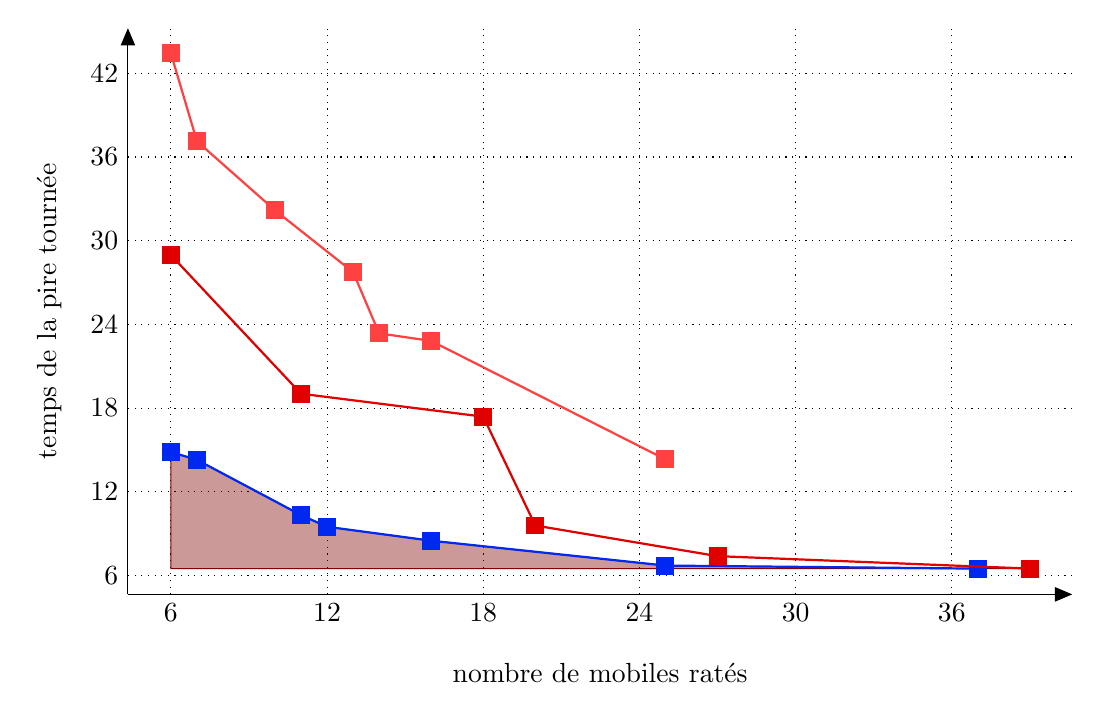
\begin{tikzpicture}[xscale=0.330579,yscale=0.17711]
\draw[xstep=6,ystep=6,thin,dotted,color=Black] (4.35,4.6401) grid (40.6267,45.2371);
\begin{scope}
  \clip (4.35,4.6401) rectangle (40.6267,45.2371);
  \definecolor{hvColor}{RGB}{128,0,0}
  \draw[color=hvColor, fill=hvColor, fill opacity=0.4] (6,6.4877) -- (6,14.8468) -- (7,14.2892) -- (11,10.3245) -- (12,9.48769) -- (16,8.48855) -- (25,6.70582) -- (37,6.4877) -| (39,6.4877) -- cycle;
  \definecolor{pLineColor}{RGB}{128,0,0}
  \definecolor{pPointColor}{RGB}{0,40,240}
  \draw[thick,color=pPointColor] (6,14.8468) node[draw,color=pPointColor,fill=pPointColor, inner sep = 0pt, minimum size=2mm] {} -- (7,14.2892) node[draw,color=pPointColor,fill=pPointColor, inner sep = 0pt, minimum size=2mm] {} -- (11,10.3245) node[draw,color=pPointColor,fill=pPointColor, inner sep = 0pt, minimum size=2mm] {} -- (12,9.48769) node[draw,color=pPointColor,fill=pPointColor, inner sep = 0pt, minimum size=2mm] {} -- (16,8.48855) node[draw,color=pPointColor,fill=pPointColor, inner sep = 0pt, minimum size=2mm] {} -- (25,6.70582) node[draw,color=pPointColor,fill=pPointColor, inner sep = 0pt, minimum size=2mm] {} -- (37,6.4877) node[draw,color=pPointColor,fill=pPointColor, inner sep = 0pt, minimum size=2mm] {};
  \definecolor{pLineColor}{RGB}{224,0,0}
  \definecolor{pPointColor}{RGB}{224,0,0}
  \draw[thick,color=pPointColor] (6,28.9739) node[draw,color=pPointColor,fill=pPointColor, inner sep = 0pt, minimum size=2mm] {} -- (11,19.0276) node[draw,color=pPointColor,fill=pPointColor, inner sep = 0pt, minimum size=2mm] {} -- (18,17.3831) node[draw,color=pPointColor,fill=pPointColor, inner sep = 0pt, minimum size=2mm] {} -- (20,9.57881) node[draw,color=pPointColor,fill=pPointColor, inner sep = 0pt, minimum size=2mm] {} -- (27,7.38144) node[draw,color=pPointColor,fill=pPointColor, inner sep = 0pt, minimum size=2mm] {} -- (39,6.4877) node[draw,color=pPointColor,fill=pPointColor, inner sep = 0pt, minimum size=2mm] {};
  \definecolor{pLineColor}{RGB}{255,65,65}
  \definecolor{pPointColor}{RGB}{255,65,65}
  \draw[thick,color=pPointColor] (6,43.4396) node[draw,color=pPointColor,fill=pPointColor, inner sep = 0pt, minimum size=2mm] {} -- (7,37.1319) node[draw,color=pPointColor,fill=pPointColor, inner sep = 0pt, minimum size=2mm] {} -- (10,32.1803) node[draw,color=pPointColor,fill=pPointColor, inner sep = 0pt, minimum size=2mm] {} -- (13,27.7482) node[draw,color=pPointColor,fill=pPointColor, inner sep = 0pt, minimum size=2mm] {} -- (14,23.3577) node[draw,color=pPointColor,fill=pPointColor, inner sep = 0pt, minimum size=2mm] {} -- (16,22.8144) node[draw,color=pPointColor,fill=pPointColor, inner sep = 0pt, minimum size=2mm] {} -- (25,14.3196) node[draw,color=pPointColor,fill=pPointColor, inner sep = 0pt, minimum size=2mm] {};
\end{scope}
\draw[->,>=triangle 45] (4.35,4.6401) -- coordinate (x axis mid) (40.6267,4.6401);
\node[below=1cm,anchor=center] at (x axis mid) {nombre de mobiles ratés};
\foreach \x in {6,12,18,24,30,36}
  \draw (\x,4.6401) -- (\x,4.6401) node[anchor=north] {\x};
\draw[->,>=triangle 45] (4.35,4.6401) -- coordinate (y axis mid) (4.35,45.2371);
\node[left=1cm,rotate=90,anchor=center] at (y axis mid) {temps de la pire tournée};
\foreach \y in {6,12,18,24,30,36,42}
  \draw (4.35,\y) -- (4.35,\y) node[anchor=east] {\y};
\end{tikzpicture}
\end{document}
